\input{/home/nick/latex-preambles/xelatex.tex}

\newcommand{\imagesPath}{.}

\title{
	\textbf{Δίκτυα Υπολογιστών} \\~\\
	Εργαστηριακή Άσκηση 6 \\ 
	Πρωτόκολλο ICMP 
}
\author{}
\date{}

\begin{document}
	\maketitle
	
	\begin{tabular}{|l|l|}
		\hline
		\textbf{Ονοματεπώνυμο:} Νικόλαος Παγώνας, el18175 & \textbf{Ομάδα:} 4 (Τρίτη εξ' αποστάσεως) \\
		\hline
		\textbf{Όνομα PC/ΛΣ:} nick-ubuntu/Ubuntu 20.04.3 LTS & \textbf{Ημερομηνία:} Τρίτη 23/11/2021\\
		\hline
		\textbf{Διεύθυνση IP:} \verb|192.168.1.15| & \textbf{Διεύθυνση MAC:} \verb|3c:2c:30:e1:1c:55|\\
		\hline
	\end{tabular}

	\section*{1 - Εντολή ping στο τοπικό υποδίκτυο}
		Εκτελέσαμε την εντολή  \verb|ping 192.168.1.7|.
		
		\subsection*{1.1}
			To φίλτρο σύλληψης που χρησιμοποιήσαμε είναι \verb|ether host 3C:2C:30:E1:1C:55|.
		
		\subsection*{1.2}
			Το φίλτρο απεικόνισης που χρησιμοποιήσαμε είναι \verb+arp || icmp+.
		
		\subsection*{1.3}
			Ο σκοπός των πακέτων ARP που ανταλλάχθηκαν είναι να βρεθεί σε ποια MAC address αντιστοιχεί η IPv4 διεύθυνση 192.168.1.7.
		
		\subsection*{1.4}
			Το πεδίο που προσδιορίζει ότι πρόκειται για μήνυμα ICMP είναι το \verb|Protocol|, και έχει τιμή \verb|0x01|.
	
		\subsection*{1.5}
			Το μήκος της επικεφαλίδας των μηνυμάτων ICMP Echo Request είναι 8 bytes.
	
		\subsection*{1.6}
			\begin{itemize}
				\item Type: 1 byte 
				\item Code: 1 byte
				\item Checksum: 2 bytes
				\item Identifier: 2 bytes
				\item Sequence Number: 2 bytes
			\end{itemize}
			
			\begin{figure}[H]
				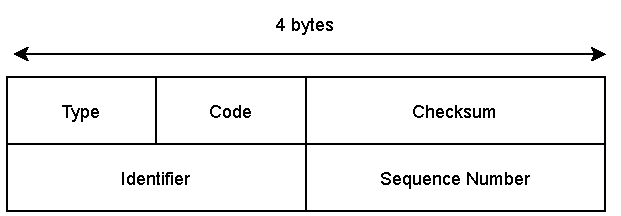
\includegraphics[width=0.6\linewidth]{\imagesPath/1.6.pdf}
			\end{figure}
	
		\subsection*{1.7}
			\begin{itemize}
				\item Type: 0x08
				\item Code: 0x00
			\end{itemize}
	
		\subsection*{1.8}
			\begin{itemize}
				\item Identifier: 0x0001
				\item Sequence Number: 0x0001
			\end{itemize}
	
		\subsection*{1.9}
			Το μήκος του πεδίου δεδομένων είναι 48 bytes, ενώ το περιεχόμενο είναι: \\
			
			2f02040000000000101112131415161718191a1b1c1d1e1f202122232425262728292a2b2c2d2e2f3031323334353637. \\
			
			Παρατηρούμε ότι μετά από ένα σημείο έχουμε byte που είναι διαδοχικά μεταξύ τους (10, 11, 12, ...).
	
		\subsection*{1.10}
			Τόσο το μήκος όσο και η δομή της επικεφαλίδας ενός μηνύματος ICMP Echo reply είναι ίδια με το ICMP Echo request.  
	
		\subsection*{1.11}
			\begin{itemize}
				\item Type: 0x00
				\item Code: 0x00
			\end{itemize}
	
		\subsection*{1.12}
			Το πεδίο Type καθορίζει το είδος του μηνύματος, αφού αυτό είναι που διαφέρει μεταξύ των δύο περιπτώσεων.
	
		\subsection*{1.13}
			\begin{itemize}
				\item Identifier: 0x0001
				\item Sequence Number: 0x0001
			\end{itemize}
	
		\subsection*{1.14}
			\begin{itemize}
				\item Identifier: 0x0001
				\item Sequence Number: 0x0001
			\end{itemize}
		
			Παρατηρούμε ότι τα πεδία έχουν ίδιες τιμές στο Request και στο Reply.
	
		\subsection*{1.15}
			Τα πεδία αυτά χρησιμοποιούνται προκειμένου να γίνει η αντιστοίχιση μεταξύ request και reply.
	
		\subsection*{1.16}
			Μήκος 48 bytes, περιεχόμενο πεδίου δεδομένων: \\
			
			2f02040000000000101112131415161718191a1b1c1d1e1f202122232425262728292a2b2c2d2e2f3031323334353637. \\ 
			
			Πάλι έχουμε διαδοχικά byte (10, 11, 12, ...).
	
		\subsection*{1.17}
			Όχι, είναι το ίδιο.
	
		\subsection*{1.18}
			Κάθε ανταλλαγή ICMP Request/Reply αντιστοιχεί και σε μία γραμμή που τυπώνει η ping στο παράθυρο εντολών.
	
		\subsection*{1.19}
			Στέλνουμε στην ίδια συσκευή με διεύθυνση 192.168.1.7, αλλά τώρα της έχουμε απενεργοποιήσει το ίντερνετ. \\
			Χρησιμοποιήσαμε την εντολή \verb|ping -c 2 192.168.1.7|.
	
		\subsection*{1.20}
			Στάλθηκαν:
			\begin{itemize}
				\item 1 πακέτο ARP "Who has 192.168.1.15? Tell 192.168.1.1"
				\item 1 πακέτο ARP "192.168.1.15 is at 3c:2c:30:e1:1c:55"
				\item 4 πακέτα ARP "Who has 192.168.1.7? Tell 192.168.1.15".	
			\end{itemize} 
	
		\subsection*{1.21}
			Τα τελευταία 4 πακέτα στέλνονται ανά 1 sec περίπου.
	
		\subsection*{1.22}
			Δεν στάλθηκε κανένα πακέτο ICMP.
	
		\subsection*{1.23}
			Παρατηρούμε από το παράθυρο εντολών ότι έγινε προσπάθεια να σταλούν 2 πακέτα, αλλά "χάθηκαν" και τα 2, δηλαδή δεν είχαμε επιτυχή αποστολή.
	
	\section*{2 - Εντολή ping σε άλλο υποδίκτυο}
	
		\subsection*{2.1}
			Κάνουμε \verb|ip neigh flush all| για να φανούν ξεκάθαρα οι διευθύνσεις IPv4 που θα προκύψουν μετά το ping. Στην συνέχεια κάνουμε \verb|ping 147.102.1.1|. Με την εντολή \verb|ip neigh| καταγράφουμε τις διευθύνσεις 192.168.1.1 και 192.168.1.9.
	
		\subsection*{2.2}
			\begin{itemize}
				\item Source: \verb|3c:2c:30:e1:1c:55| 
				\item Destination: \verb|e0:0e:e4:59:40:50|
			\end{itemize}
			
	
		\subsection*{2.3}
			\begin{itemize}
				\item Source: \verb|192.168.1.15|
				\item Destination: \verb|147.102.1.1|
			\end{itemize}
	
		\subsection*{2.4}
			Η διεύθυνση \verb|3c:2c:30:e1:1c:55| αντιστοιχεί στην \verb|192.168.1.15|, δηλαδή στο μηχάνημά μας, ενώ η \verb|e0:0e:e4:59:40:50| αντιστοιχεί στην \verb|192.168.1.1|, δηλαδή στην διεύθυνση του router μας.
	
		\subsection*{2.5}
			Ναι, παρατηρήσαμε.
	
		\subsection*{2.6}
			Επειδή είχαμε κάνει flush τον πίνακα arp, έπρεπε να γίνει η αντιστοίχιση των IPv4 διευθύνσεων σε διευθύνσεις MAC. Επομένως είναι λογικό να εμφανιστούν πακέτα ARP κατά την καταγραφή.
	
		\subsection*{2.7}
			Επειδή τα ICMP Echo replies έχουν Type = 0, το φίλτρο θα είναι \verb|icmp.type == 0|.
	
		\subsection*{2.8}
			Επειδή η default τιμή του TTL ακριβώς μόλις φεύγουν τα πακέτα είναι 64, και η τιμή που βλέπουμε με το Wireshark είναι 58, αυτό σημαίνει ότι η διεύθυνση Η διεύθυνση 147.102.1.1 είναι 7 hops μακριά (μπορούμε να το επιβεβαιώσουμε και με την traceroute).
	
		\subsection*{2.9}
			Εμφανίζονται \verb|ICMP echo ping request| και \verb|ICMP destination unreachable (port unreachable)|.
	
		\subsection*{2.10}
			Στην περίπτωση που κάναμε ping στο μηχάνημα του υποδικτύου μας, τα πακέτα ICMP δεν έφυγαν ποτέ, αφού χρειαζόταν η MAC address του μηχανήματος. Αντίθετα, όταν κάνουμε ping σε ανενεργό υπολογιστή εκτός του υποδικτύου μας, τα πακέτα ICMP πηγαίνουν στο router, άσχετα αν στη συνέχεια δεν θα βρουν τον προορισμό, οπότε παρατηρείται η κίνησή τους. 
	
	\section*{3 - Εντολή tracert/traceroute}
	
		\subsection*{3.1}
			Το μήκος είναι 32 bytes και το περιεχόμενο είναι: \\ 
			
			48494a4b4c4d4e4f505152535455565758595a5b5c5d5e5f6061626364656667 \\
			
			(αυξανόμενοι δεκαεξαδικοί αριθμοί από το 48 μέχρι και το 67).
	
		\subsection*{3.2}
			Στο 1.9 είχαμε 48 bytes, ενώ τώρα έχουμε 32.
	
		\subsection*{3.3}
			Time-to-live exceeded (Time to live exceeded in transit)
	
		\subsection*{3.4}
			Type: 0x0b (Time-to-live exceeded), Code: 0x00 (Time to live exceeded in transit)
	
		\subsection*{3.5}
			\begin{itemize}
				\item Checksum: 2 bytes
				\item Unused: 1 byte
				\item Length: 1 byte
				\item Unused: 2 bytes
			\end{itemize}
			
		\subsection*{3.6}
			Μήκος επικεφαλίδας 8 bytes, Μήκος δεδομένων 68 bytes.
	
		\subsection*{3.7}
			Το περιεχόμενο είναι το IP Header του πακέτου που προκάλεσε το σφάλμα, καθώς και ένα μέρος (τα leading octets) των δεδομένων του. 

	\section*{4 - Ανακάλυψη MTU διαδρομής (Path MTU Discovery)}

		\subsection*{4.1}
			Οι τιμές πεδίου δεδομένων που θα χρησιμοποιήσουμε είναι 1472, 1464, 978, 548, 524, 516, 484, 480, 268, κατά 28 byte μικρότερες από το μέγεθος πακέτων IPv4 που αναγράφονται στην εκφώνηση (επειδή το IP header είναι 20 bytes και το ICMP Header 8 bytes).   

		\subsection*{4.2}
			Ναι, παρατηρήσαμε.

		\subsection*{4.3}
			Το παρήγαγε ο κόμβος με IPv4 διεύθυνση 192.168.1.1, δηλαδή το router μας.

		\subsection*{4.4}
			\begin{itemize}
				\item Type: 0x03 (Destination Unreachable)
				\item Code: 0x04 (Fragmentation Needed)
			\end{itemize}

		\subsection*{4.5}
			To πεδίο \verb|Fragmentation needed| δείχνει ότι χρειαζόταν θρυμματισμός, ενώ το πεδίο \verb|MTU of next hop| είναι 1492.

		\subsection*{4.6}
			Περιέχει την επικεφαλίδα IPv4, την επικεφαλίδα ICMP και 520 bytes ICMP Data από το πακέτο που έλαβε ο κόμβος που στέλνει το μήνυμα Destination Unreachable.

		\subsection*{4.7}
			Είναι 1492 bytes.

		\subsection*{4.8}
			Συνολικά δεν απαντά για τις τιμές 1500 (προφανώς αφού ξεπερνά το MTU) αλλά και για τις τιμές 1492 και 1006.

		\subsection*{4.9}
			Η τιμή MTU για την οποία λαμβάνουμε απάντηση είναι 576 bytes.

		\subsection*{4.10}
			Αν κάνουμε ping με καταγραφή διαδρομής μέχρι τον 147.102.40.15 και μετά κάνουμε ping σε όλους τους ενδιάμεσους κόμβους, με απαίτηση μη θρυμματισμού και με μέγεθος πακέτου IPv4 1006 (το αμέσως μεγαλύτερο από το 576), τότε βρίσκουμε ότι ο πρώτος κόμβος που δεν απαντά είναι ο 147.102.40.15, άρα η MTU είναι του 147.102.40.15.

		\subsection*{4.12}
			Δεν παρατηρήσαμε θρυμματισμό.
 
	\section*{5 - Απρόσιτη Θύρα (Port Unreachable)}

		\subsection*{5.1}
			Χρησιμοποιήσαμε φίλτρο σύλληψης \verb|ip && host 147.102.40.15|.

		\subsection*{5.2}
			Η σύνταξη της εντολής που χρησιμοποιήσαμε είναι: \verb|dig -4 @147.102.40.15 edu-dy.cn.ntua.gr|

		\subsection*{5.3}
			Λάβαμε την εξής απάντηση: connection timed out; no servers could be reached
			
			\begin{figure}[H]
				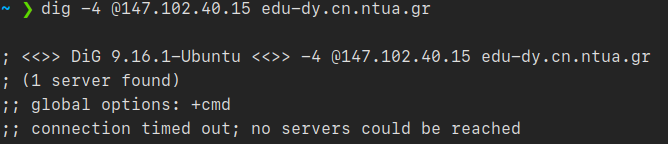
\includegraphics[width=\linewidth]{\imagesPath/5.3.png}
			\end{figure}

			Αυτό σημαίνει ότι το request δεν έφτασε στον εξυπηρετητή DNS του 147.102.40.15.
			  
		\subsection*{5.4}
			Ναι, παρατηρήσαμε.

		\subsection*{5.5}
			Το πρωτόκολλο μεταφοράς είναι το UDP και η θύρα προορισμού είναι η 53.

		\subsection*{5.6}
			Ναι παρατηρήσαμε.

		\subsection*{5.7}
			\begin{itemize}
				\item Type: 0x03
				\item Code: 0x03
			\end{itemize}

		\subsection*{5.8}
			Το πεδίο Code. 

		\subsection*{5.9}
			Επειδή η θύρα 53 είναι προκαθορισμένη για αιτήματα DNS.

		\subsection*{5.10}
			Έχουμε δει από την Εργαστηριακή Άσκηση 5 ότι o προορισμός απαντά με Destination Unreachable (Port Unreachable).
	
	\section*{6 - IPv6 και ICMPv6}

		\subsection*{6.1}
			Η σύνταξη των εντολών είναι: \\
			
			\verb|ping -6 -c 1 2001:648:2000:329::101| \\
			\verb|traceroute -6 -I 2001:648:2000:329::101 |

		\subsection*{6.2}
			To φίλτρο σύλληψης είναι \verb|ip6| και το φίλτρο απεικόνισης είναι \verb|icmpv6|. 

		\subsection*{6.3}
			Το πεδίο Type έχει τιμή \verb|0x86dd|.

		\subsection*{6.4}
			Το μήκος της επικεφαλίδας IPv6 είναι 40 bytes.

		\subsection*{6.5}
			\begin{itemize}
				\item Version: 4 bits
				\item Traffic Class: 8 bits 
				\item Flow Label: 20 bits
				\item Payload Length: 16 bits
				\item Next Header: 8 bits
				\item Hop Limit: 8 bits
				\item Source Address: 16 bytes
				\item Destination Address: 16 bytes
			\end{itemize}
		
			\begin{figure}[H]
				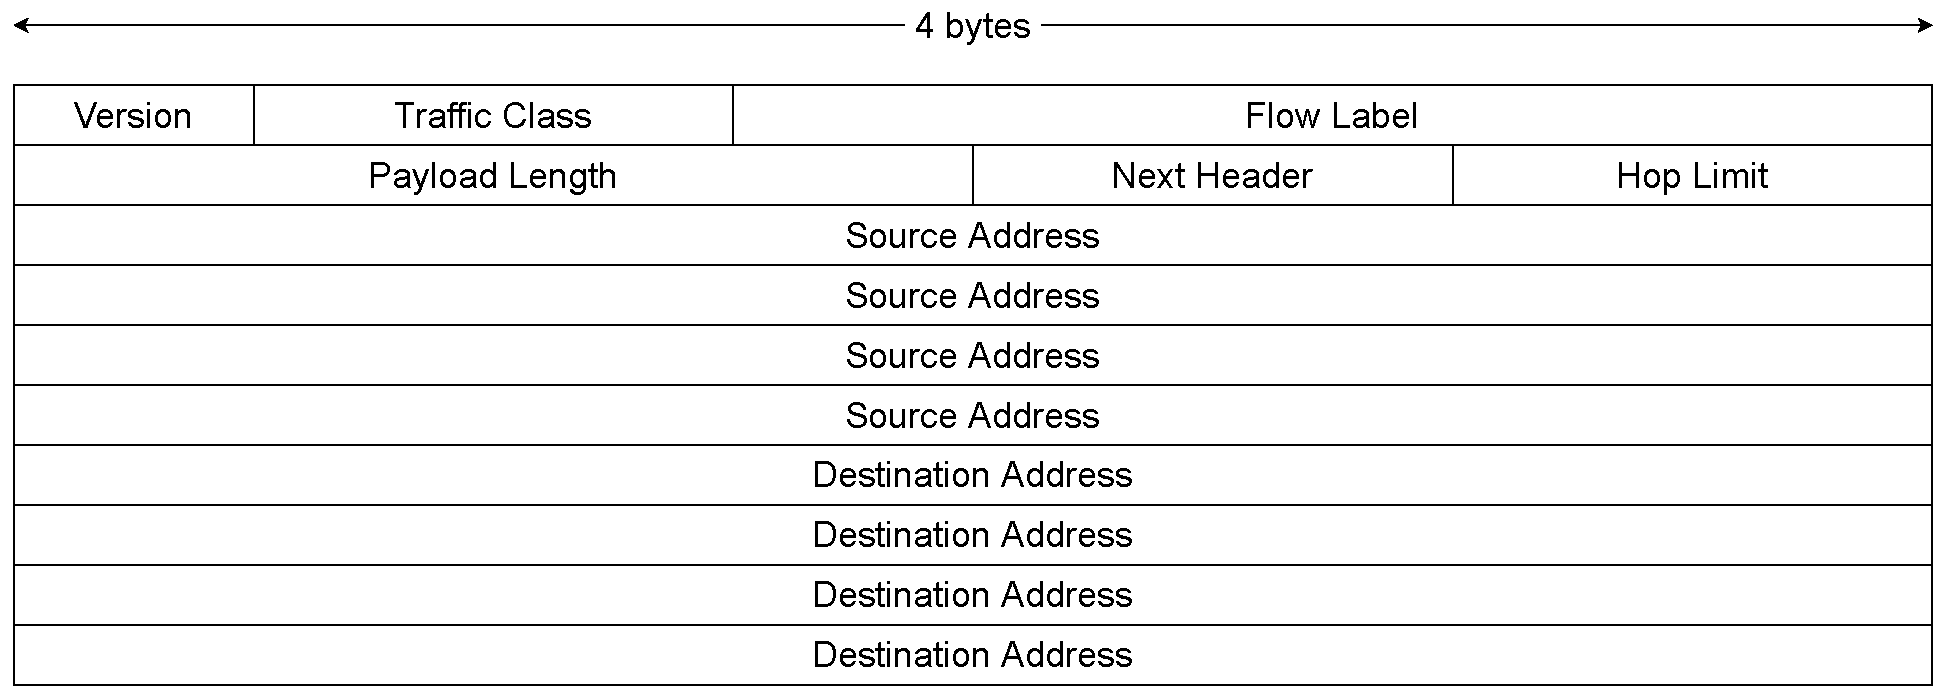
\includegraphics[width=\linewidth]{\imagesPath/6.5.pdf}
			\end{figure}
			
		\subsection*{6.6}
			Η αντίστοιχη της TTL είναι η επικεφαλίδα Hop Limit.

		\subsection*{6.7}
			Η επικεφαλίδα Next Header, για το ICMPv6 η τιμή της είναι 58.

		\subsection*{6.8}
			Ναι, είναι ίδια.

		\subsection*{6.9}
			Type: Echo (ping) request (128), μήκος δεδομένων: 56 bytes

		\subsection*{6.10}
			Ναι, είναι ίδια.

		\subsection*{6.11}
			type: Echo (ping) reply (129), μήκος δεδομένων: 56 bytes

		\subsection*{6.12}
			Διαφέρει στα πεδία Payload Length (άρα και στο μέγεθος των ICMP Data), και στο πεδίο Hop Limit (αφού αρχικά η traceroute στέλνει πακέτα με μικρό Hop Limit και στη συνέχεια στέλνει πακέτα με σταδιακά μεγαλύτερο Hop Limit).

		\subsection*{6.13}
			Η δομή είναι ίδια, εκτός από το ότι έχουμε το πεδίο Reserved αντί για το πεδίο Unused.

		\subsection*{6.14}
			Η τιμή του πεδίου Type είναι 3 και το μήκος δεδομένων είναι 80 bytes.

		\subsection*{6.15}
			Περιέχει τα IPv6 και ICMPv6 headers, καθώς και τα δεδομένα του μηνύματος που ελήφθη.

		\subsection*{6.16}
			Παρατήρησα μηνύματα ICMPv6 Neighbor Advertisement/Solicitation.

		\subsection*{6.17}
			 Τα μηνύματα Neighbor Advertisement έχουν μήκος 24 ή 32 bytes και Type = 136, ενώ τα Neighbor Solicitation έχουν μέγεθος 32 bytes και Type = 135.
\end{document}